\section{Random forest}
El random forest es una técnica de machine learning de uso común, este algoritmo combina el resultado de múltiples arboles de desición para llegar a un resultado único. \\
Es una técnica fácil de interpretar, estable y que por lo general presenta buenas coincidencias y que se puede utilizar en tareas de regresión o clasificación. \\
Esta técnica de machine learning se utiliza ampliamente ya que reduce el riesgo de sobre ajuste, maneja datos grandes y con ruido, es escalable, versátil y menos sensible a datos atípicos.
\section{Metodologia}
El código del programa se ejecuto en un google collab, duplicando el notebook que el documento "AprendeMachineLearning" proporciona\\
Cuando los datos están listos para ejecutarse, usamos la siguiente función para entrenarlo con los datos dados
\begin{figure}[H]
    \centering
    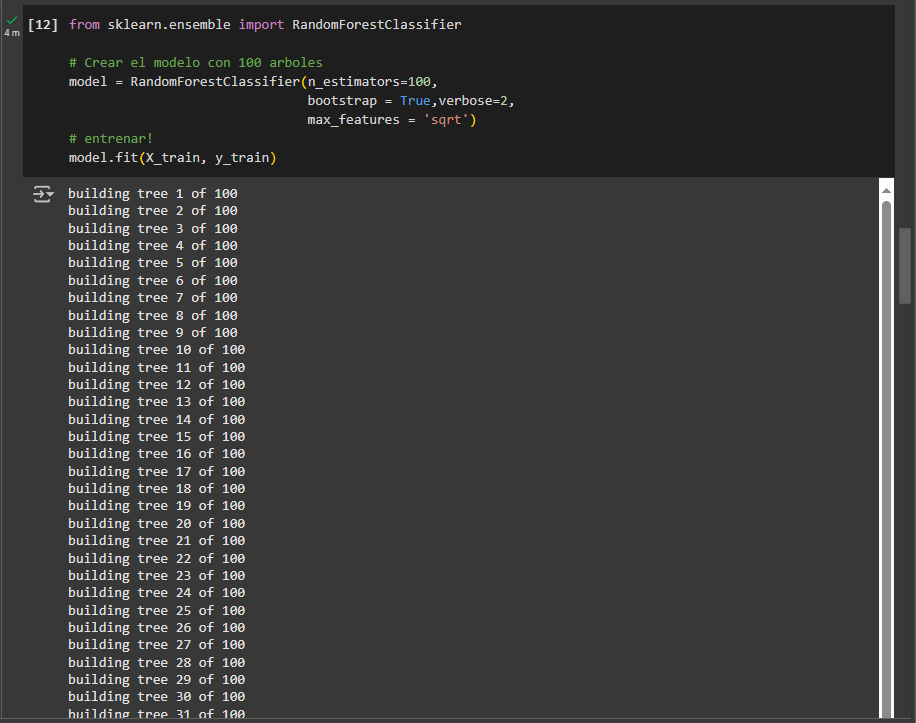
\includegraphics[width=0.75\linewidth]{image.png}
\end{figure}
\newpage
Después de esto se utiliza otro random forest mas veloz
\begin{figure}[H]
    \centering
    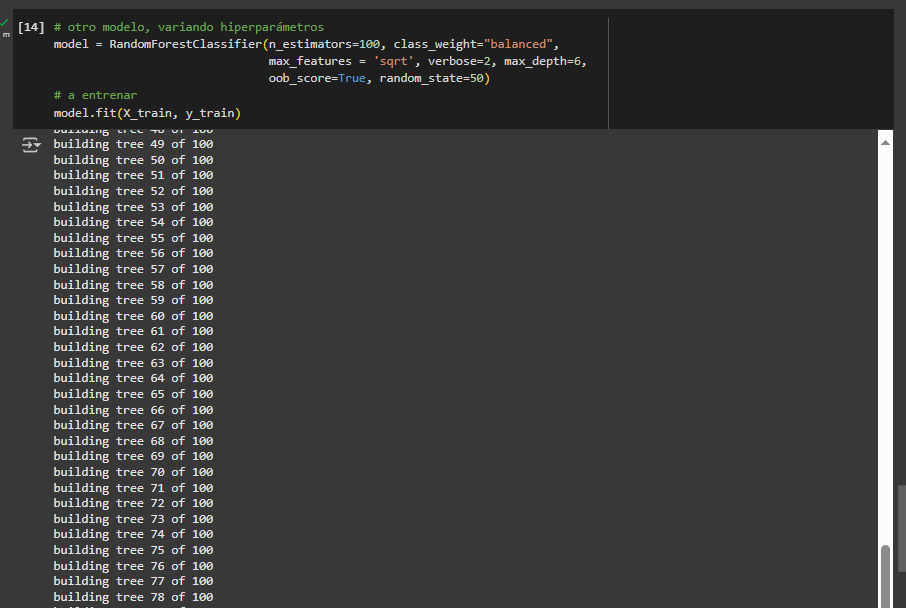
\includegraphics[width=0.5\linewidth]{image2.png}
\end{figure}

\section{Resultados}
El test nos dio la siguiente matriz
\begin{figure}[H]
    \centering
    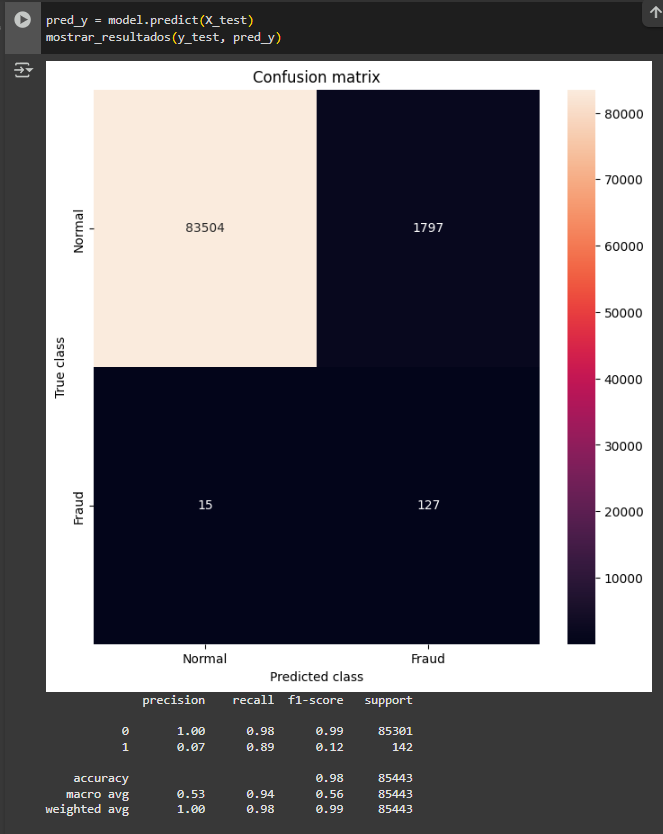
\includegraphics[width=0.5\linewidth]{matriz0.png}
\end{figure}
Se obtuvo un desempeño bueno considerando que es un test y que no se ha entrenado aun al modelo con el random forest
El segundo modelo nos dio la siguiente matriz:
\begin{figure}[H]
    \centering
    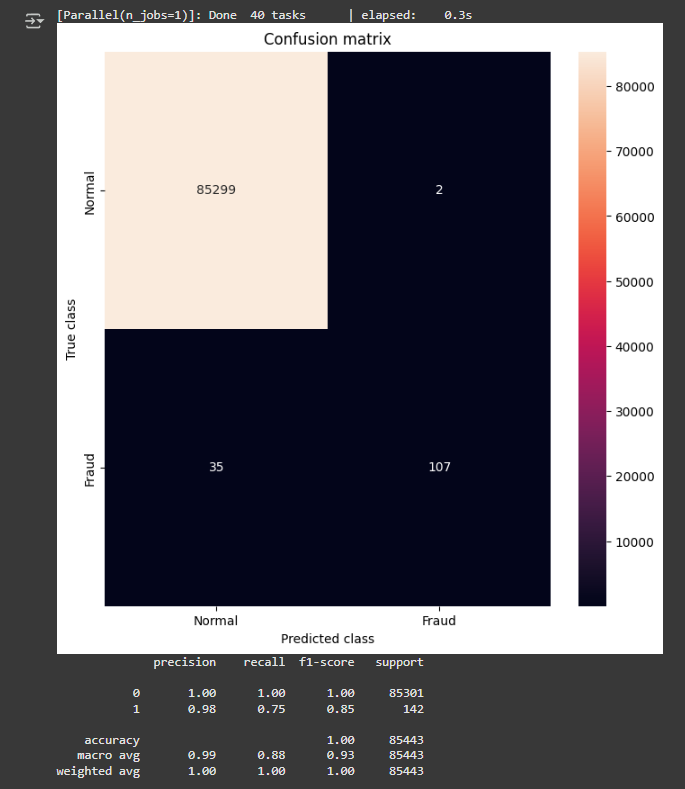
\includegraphics[width=0.5\linewidth]{matriz1.png}
\end{figure}
Este modelo tuvo un desempeño bastante mejor ya que clasifico menos normales como fraudes a comparacion del test.\\
Por ultimo con el ultimo modelado, usando un random forest mas rápido
\begin{figure}[H]
    \centering
    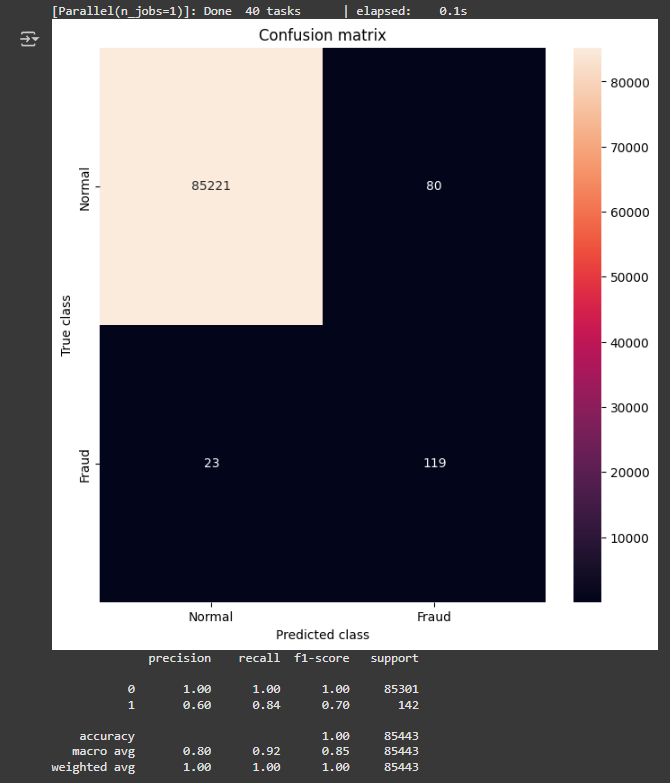
\includegraphics[width=0.5\linewidth]{matriz2.png}
\end{figure}
Se obtuvieron resultados mejores que en el test, pero que no son tan buenos como los del segundo modelo.


\section{Conclusión}
Aprendi mas acerca de los random forest, como se utilizan y para que sirven, ya que aun que ya conocía cosas del machine learning, no sabia de los random forest, ademas con esta practica pude observar por mi mismo como cambia la eficacia del método cambiando la forma en la que el random forest trabaja con los datos.
